\documentclass[11pt]{article}
\usepackage[margin=1in]{geometry}
\usepackage{booktabs}
\usepackage{amsmath,amssymb}
\usepackage{tabularx}
\usepackage{microtype}
\usepackage{xspace}
\usepackage{tikz}
\usetikzlibrary{positioning,arrows.meta,calc}
\usepackage{pgfplots}
\pgfplotsset{compat=1.18}
\usepgfplotslibrary{groupplots}
\usetikzlibrary{patterns}
% Figure palette: one hue per framework (validated categorical pair; CVD dE 24.7,
% normal-vision dE 33.6, >=3:1 on white), neutral inks for all text and chrome.
\definecolor{sglang}{HTML}{2A78D6}
\definecolor{vllm}{HTML}{EB6834}
\definecolor{inksec}{HTML}{52514E}
\definecolor{inkmuted}{HTML}{898781}
\definecolor{gridc}{HTML}{E1E0D9}
\definecolor{axisc}{HTML}{C3C2B7}
\definecolor{panel}{HTML}{F5F4F0}
\usepackage[numbers,sort&compress]{natbib}
\usepackage[hidelinks]{hyperref}
\hypersetup{pdftitle={No Permanent Champion: A Deployment Study of SGLang and vLLM across Dense, Ultra-Sparse MoE, and KDA-Hybrid Architectures on H200 GPUs}, pdfauthor={Chao-Chun Chuang, Po-Hsiang Lin}}
\usepackage{url}

\newcommand{\tps}{tok/s\xspace}
\newcommand{\figsub}[1]{{\footnotesize\color{inksec}#1}}

\title{\textbf{No Permanent Champion: A Deployment Study of SGLang and vLLM across Dense, Ultra-Sparse MoE, and KDA-Hybrid Architectures on H200 GPUs}}

\author{
Chao-Chun Chuang$^{1,\ast}$ and Po-Hsiang Lin$^{2}$\\[4pt]
\small $^{1}$National Center for High-performance Computing (NCHC),\\
\small National Institutes of Applied Research (NIAR), Taiwan\\
\small $^{2}$Kaohsiung Veterans General Hospital, Kaohsiung, Taiwan\\[2pt]
\small $\ast$ Corresponding author: \texttt{c00cjz00@nchc.org.tw}
}
\date{September 2026}

\begin{document}
\maketitle

\begin{abstract}
\noindent We operate a multi-model API service on an HPC cluster---a LiteLLM gateway fronting Slurm-managed SGLang and vLLM engines on NVIDIA H200 GPUs---and each new model it onboards raises the same question: which serving framework will run this checkpoint faster? We encoded an A/B comparison procedure as versioned procedures (``skills'') that an LLM-based agent executed under human approval: scaffolding both frameworks' engines from official per-model documentation, deploying them under traffic-isolated aliases, and driving the same single-burst 500--1,000-user workload at each, with aggregate output-token counts compared per run. Applied to three 2026 models---a 27B dense hybrid, a 180B-total/6B-active ultra-sparse MoE, and a 288-expert Kimi Delta Attention (KDA) hybrid MoE---the observed leader changed each time: SGLang led by 6.3\% (near parity) on the dense model, vLLM by 2.33$\times$ on the MoE, and SGLang by 28\% on the KDA hybrid. Speculative decoding on the same checkpoints reduced measured throughput in five of six framework--model pairs (single-run burst measurements) and cut one run's success rate to 85.6\%; disabling it on the production engine gained 17--20\% the same day. An agent-assisted layered diagnosis, encoded as a symptom-to-cause procedure, raised mixed 1,500-user success from 67.9\% to 100\% by correcting file-descriptor limits. These observations indicate that framework choice and speculative decoding should be measured per model rather than inherited as defaults; the procedure is a versioned artifact of our repository.
\end{abstract}

\section{Introduction}

The throughput and latency of a deployed large language model (LLM) depend not only on the model and the accelerator, but on the serving framework that schedules batches, manages KV-cache memory, and executes attention and mixture-of-experts (MoE) kernels. Among the open-source frameworks used for self-hosted deployment, vLLM is the most widely adopted in practice and SGLang is among its principal alternatives~\cite{majidi2026wild}. vLLM was introduced with PagedAttention for efficient KV-cache memory management~\cite{kwon2023vllm}, and SGLang with a RadixAttention prefix cache and a structured-generation runtime~\cite{zheng2024sglang}. Both systems evolve quickly, add support for new model architectures as they appear, and make different implementation trade-offs for the same architecture. Practitioners therefore face a recurring question that vendor documentation does not answer: \emph{for this specific model, on this hardware, which framework will serve it faster?}

This question is not academic for us. We operate a multi-model API service for the users of an HPC cluster: a LiteLLM gateway fronting Slurm-managed inference engines---SGLang and vLLM containers among them---on NVIDIA H200 GPUs, with per-engine lifecycle management, versioned container images, and declarative routing that lets a candidate engine receive production-shaped traffic under isolated aliases before it claims any production name. Every time the center onboards a new open-weight model, the platform forces a concrete framework decision, and the wrong one is expensive: as this paper shows, the cost of choosing wrongly reaches 2.3$\times$ in throughput---larger than any tuning lever we measured, including correcting an outright misconfiguration (+48\% on the dense engine's earlier settings). Manual evaluation is slow and error-prone (framework-specific flags, memory budgets, and validation steps differ), so we delegated it to an agent: the evaluation procedure---engine scaffolding from each framework's official per-model documentation, dual-framework deployment, paired benchmarking, verdict recording, and production traffic switching---was encoded as declarative, versioned procedures (which we call \emph{skills}) and executed by an LLM-based coding agent under human approval. Each framework decision in this study was completed within a day; we did not measure the agent's unattended time or the labor it saved.

Published comparisons between serving systems do exist: an empirical evaluation of vLLM against HuggingFace TGI on LLaMA-2 models is a recent example~\cite{kolluru2025tgi}, surveys consolidate the serving-systems literature~\cite{li2024survey}, and a study of open-source deployments documents which frameworks practitioners actually adopt~\cite{majidi2026wild}. Same-checkpoint comparisons of multiple backends have quantified accuracy fidelity~\cite{pape2026silent}, and SiliconBench evaluates nine Apple Silicon serving engines on unified-memory desktops, using CUDA vLLM and SGLang as references~\cite{zhang2026siliconbench}; neither addresses throughput at hundreds to a thousand concurrent requests on HPC GPUs, and none evaluates ultra-sparse MoE or KDA hybrids. Separately, the fragility of speculative decoding under batched serving is not merely a vendor warning: goodput analyses and adaptive speculation control have formalized when drafting helps and when it hurts~\cite{liu2024turbospec,li2025adaserve}. What remains unmeasured is how these framework and speculation choices behave on the newest architectures---with checkpoint-integrated multi-token prediction (MTP) heads rather than external draft models---under high-concurrency burst load.

The present paper reports what this agent-assisted workflow found, together with the workflow itself. We make four contributions:

\begin{enumerate}
\item \textbf{An agent-assisted evaluation workflow} (Sections~3--4): a paired A/B procedure---both frameworks serving the \emph{same local checkpoint} on the same GPU type under the \emph{same client workload}, engine parameters taken from official documentation, and aggregate output-token counts compared and disclosed pair by pair---encoded as versioned skills that an LLM-based agent executed under human approval, from scaffolding the candidate engine to switching production traffic when the verdict is in.
\item \textbf{Three per-model observations} (Section~5): SGLang 0.5.20 led by 6.3\% (near parity) on a dense 27B hybrid; vLLM 0.29.1rc1 led by 2.33$\times$ on a 180B/6B-active ultra-sparse MoE; SGLang led by 28\% on a 306 GB FP8 KDA model---indicating that the leading framework is model-specific, with differences large enough (up to 2.3$\times$) to outweigh the other tuning levers we measured.
\item \textbf{A negative result for speculative decoding under load}: across the three models and two frameworks (six framework--model pairs), speculative decoding reduced aggregate throughput in five cases (by 15--46\%) and, in the worst case, degraded the request success rate to 85.6\% through timeouts; one verdict was applied to production the same day (+17--20\%).
\item \textbf{A production platform description and reliability analysis} (Sections~3 and~5.5): a LiteLLM-based multi-engine gateway with Slurm-managed engine lifecycle, declarative production/staging traffic switching, and versioned container images, together with a layered diagnosis---also agent-assisted, from an encoded symptom-to-cause procedure---that traced mixed-load failures (67.9\% $\rightarrow$ 91.8\% $\rightarrow$ 100\%) to file-descriptor limits in the client shell and per-connection sshd, not to GPU engines or the gateway.
\end{enumerate}

All experiments were run in September 2026 on the platform described in Section~3; raw per-run statistics are released with the platform repository.

\section{Related Work}

\textbf{Serving systems.} Iteration-level scheduling and continuous batching were introduced by Orca~\cite{yu2022orca} and adopted by vLLM, whose PagedAttention brought operating-system-style page management to KV-cache memory~\cite{kwon2023vllm}. SGLang contributed RadixAttention for automatic prefix reuse and an efficient runtime for structured generation programs~\cite{zheng2024sglang}. Chunked prefill, proposed in SARATHI, mitigates the interference of long prefills with decodes~\cite{agrawal2023sarathi}, and DistServe shows that disaggregating prefill from decoding improves goodput under latency constraints~\cite{zhong2024distserve}. Kernel libraries such as FlashInfer supply portable attention and decoding kernels that both frameworks integrate~\cite{ye2025flashinfer}. Our work does not propose a new serving mechanism; it measures two mature frameworks on a production platform and finds that their relative standing differed across the three models tested.

\textbf{Model architectures under test.} The three models we evaluate span the current design space of efficient open-weight LLMs. Qwen3.8-27B continues the dense hybrid line of Qwen3~\cite{yang2025qwen3}, combining gated delta net (GDN) linear attention with full attention. Qwen3.8-Flash-Next is an ultra-sparse MoE (180B total, 6B active parameters, 512 experts) with a large N-gram embedding table, in the lineage of DeepSeek-V2/V3's economical MoE and multi-head latent attention (MLA) designs~\cite{deepseek2024v3,deepseek2024v2}. GLM-5.3-Flash continues the GLM agentic line~\cite{glm2026glm5} as a native-FP8, 288-expert MoE (8 experts active per token, one shared expert, first three layers dense) whose 45-layer attention stack interleaves, three-to-one, 34 Kimi Delta Attention (KDA) linear-attention layers---the architecture introduced by Kimi Linear~\cite{kimi2025linear}---with 11 DeepSeek Sparse Attention (DSA) layers, plus a 1M-token context window; its closest published relatives include Kimi K2's large sparse-MoE design~\cite{kimi2025k2}, and serving-side research on KDA-style hybrids is already emerging---recurrent-state compression (DASC)~\cite{yu2026dasc}, decay-aware mixed-precision state quantization (DAMP)~\cite{zhang2026damp}, and switchable per-layer mixer placements, including KDA, served from one supernet checkpoint (Super Apriel)~\cite{slam2026superapriel}. The architectural diversity of this trio is a plausible reason framework rankings might not transfer across models---a hypothesis our results support but cannot isolate, given one model per architecture.

\textbf{Speculative decoding.} Speculative sampling accelerates autoregressive decoding by drafting multiple tokens with a cheap proposal mechanism and verifying them in parallel with the target model~\cite{leviathan2023spec}. Proposal mechanisms include additional decoding heads (Medusa~\cite{cai2024medusa}), feature-level draft models with uncertainty handling (EAGLE~\cite{li2024eagle}), and the checkpoint-integrated MTP heads of DeepSeek-V3~\cite{deepseek2024v3} and its successors, which both frameworks in this study expose as NEXTN/MTP options. The published literature evaluates speculative decoding primarily as a \emph{latency} optimization at low request concurrency~\cite{leviathan2023spec,li2024eagle,cai2024medusa}, but its behavior under batched serving has been studied: goodput analyses observe that speculation can degrade serving performance when applied without regard to load, and adaptive systems such as TurboSpec close the loop by enabling drafting only when it pays~\cite{liu2024turbospec}; AdaServe customizes speculation to per-request SLOs~\cite{li2025adaserve}. Our contribution is narrower and complementary: a systematic measurement of \emph{checkpoint-integrated} MTP/NEXTN heads across two frameworks and three architectures under high-concurrency burst load, where we find drafting to be a net cost in five of six cases.

\textbf{Empirical comparisons of serving frameworks.} A comparative performance study of vLLM and HuggingFace TGI on LLaMA-2 models (7B--70B) found framework-dependent trade-offs in throughput, latency, and memory~\cite{kolluru2025tgi}; a survey consolidates the broader serving-systems literature~\cite{li2024survey}; and a large-scale analysis of open-source systems documents which serving frameworks and methods are adopted in practice~\cite{majidi2026wild}. The Silent Hyperparameter holds weights and decoding fixed across five backends but measures accuracy reproducibility rather than throughput~\cite{pape2026silent}; SiliconBench evaluates nine Apple Silicon serving engines on unified-memory desktop hardware, using CUDA vLLM and SGLang as references, with fidelity as a first-class metric~\cite{zhang2026siliconbench}; and AutoTuneBench has agent systems auto-tune both engines under a measurement protocol stricter than ours (paired seeds, cross-run CV at most 5\%)~\cite{chen2026autotunebench}. Relative to these, our study differs in target (high-concurrency burst throughput on a production HPC platform with H200 GPUs), in scope (three 2026 hybrid architectures, including---to our knowledge---the first cross-framework serving comparison of a KDA-hybrid model~\cite{kimi2025linear}), and in the object of automation: prior agent work tunes engine configurations~\cite{chen2026autotunebench} or generates bespoke serving stacks from scratch~\cite{kamahori2026vibeserve}, whereas our skills guide an agent through the production lifecycle of an existing platform, from deployment behind a live gateway to production traffic switching.

\section{The Platform: A Production LLM Serving Stack for HPC Clusters}
\label{sec:platform}

All experiments ran on the serving platform we operate for internal users of an HPC cluster (NCHC). This section documents the platform both to establish experimental validity (Section~4) and because the platform design itself---engine lifecycle, traffic switching, and image governance---encodes operational lessons that we believe are reusable. Figure~\ref{fig:arch} outlines the request path; Table~\ref{tab:components} summarizes the components.

\begin{figure}[t]
\centering
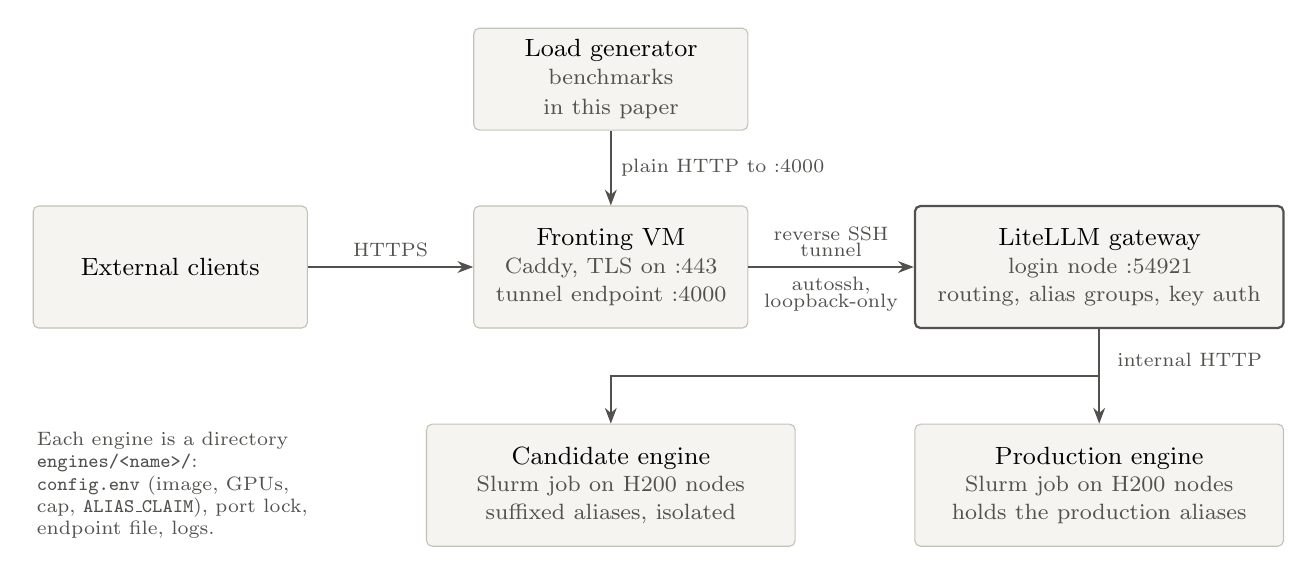
\begin{tikzpicture}[
  font=\small,
  box/.style={draw=axisc, fill=panel, rounded corners=2pt, align=center, inner sep=4pt,
              text width=3.2cm, minimum height=1.55cm,
              execute at begin node={\hyphenpenalty=10000\exhyphenpenalty=10000}},
  gw/.style={box, draw=inksec, line width=0.8pt, text width=4.4cm},
  flow/.style={-{Stealth[length=2mm]}, line width=0.7pt, draw=inksec},
  lab/.style={font=\scriptsize, text=inksec, align=center}]
\node[box] (cli) {External clients};
\node[box, right=2.1cm of cli] (vm) {Fronting VM\\[-1pt]\figsub{Caddy, TLS on :443}\\[-1pt]\figsub{tunnel endpoint :4000}};
\node[box, minimum height=0.9cm, above=0.95cm of vm] (lg) {Load generator\\[-1pt]\figsub{benchmarks in this paper}};
\node[gw, right=2.1cm of vm] (gw) {LiteLLM gateway\\[-1pt]\figsub{login node :54921}\\[-1pt]\figsub{routing, alias groups, key auth}};
\node[box, text width=4.4cm, below=1.2cm of gw] (prod) {Production engine\\[-1pt]\figsub{Slurm job on H200 nodes}\\[-1pt]\figsub{holds the production aliases}};
\node[box, text width=4.4cm] (cand) at (vm |- prod) {Candidate engine\\[-1pt]\figsub{Slurm job on H200 nodes}\\[-1pt]\figsub{suffixed aliases, isolated}};
\node[align=flush left, font=\scriptsize, text=inksec, text width=3.4cm, anchor=west,
      execute at begin node={\hyphenpenalty=10000\exhyphenpenalty=10000}] (note) at ([xshift=-2pt]cli.west |- prod)
  {Each engine is a directory \texttt{engines/<name>/}: \texttt{config.env} (image, GPUs, cap, \texttt{ALIAS\_CLAIM}), port lock, endpoint file, logs.};
\draw[flow] (cli) -- node[lab, above] {HTTPS} (vm);
\draw[flow] (lg) -- node[lab, right] {plain HTTP to :4000} (vm);
\draw[flow] (vm) -- node[lab, above] {reverse SSH\\[-2pt]tunnel} node[lab, below] {autossh,\\[-2pt]loopback-only} (gw);
\coordinate (bus) at ($(gw.south)!0.5!(prod.north)$);
\draw[line width=0.7pt, draw=inksec] (gw.south) -- (bus);
\draw[flow] (bus) -- (prod.north);
\draw[flow] (bus) -| (cand.north);
\node[lab, anchor=south west] at ([xshift=3pt]bus) {internal HTTP};
\end{tikzpicture}
\caption{Request path from external clients through the gateway to engine jobs. A candidate engine registers only suffixed aliases, so it receives benchmark traffic without claiming production names; switching which engine holds the production aliases is a two-line \texttt{ALIAS\_CLAIM} edit plus a gateway restart (Section~\ref{sec:platform}). The benchmarks in this paper entered at the tunnel's plain-HTTP endpoint on the VM, so they exercised the tunnel, gateway, and engines but not the TLS front end.}
\label{fig:arch}
\end{figure}

\begin{table}[t]
\centering
\small
\begin{tabularx}{\textwidth}{lXX}
\toprule
\textbf{Component} & \textbf{Implementation} & \textbf{Notes} \\
\midrule
Gateway & LiteLLM proxy, login node, port 54921 & 5.2\% CPU / 333 MB (observed during the 1,000-user load test) \\
Authentication & Master key + per-user virtual keys (\texttt{key\_tool.py}) & JSON key store with flock and atomic writes; no database; per-key RPM/TPM limits enforced in memory \\
Engine lifecycle & \texttt{start\_models.sh} / \texttt{stop\_models.sh} over Slurm & Idempotent dispatch, port locks, endpoint readiness files, two-stage validation (\texttt{validate\_engine.sh}) \\
Routing config & \texttt{generate\_runtime\_config.py} & Static portal models + live probing of engine endpoints; alias groups with production/isolated claims \\
Traffic switching & \texttt{ALIAS\_CLAIM} in each engine's \texttt{config.env} & Production alias set vs.\ suffixed aliases; switching frameworks = edit two lines + gateway restart ($\sim$10 s), engines keep running \\
Container images & Versioned Apptainer SIF files (\texttt{sglang\_0.5.20.sif}, \texttt{vllm\_0.29.1rc1.sif}, dedicated \texttt{vllm\_glm53-flash.sif}) & Version-named; the pull script refuses to overwrite an existing SIF unless forced, and no SIF used in this study was overwritten; dedicated vendor builds used when a model requires them; no content digests recorded \\
External access & Caddy TLS + autossh reverse tunnel, plus SSH tunnel and web-proxy paths & Loopback-only tunnel binding; IP allowlists at the fronting VM \\
\bottomrule
\end{tabularx}
\caption{Platform components.}
\label{tab:components}
\end{table}

Three design decisions deserve emphasis because they made the A/B protocol of Section~4 cheap to run and safe for production traffic. \emph{First}, engines are self-contained directories (\texttt{engines/<name>/}) whose \texttt{config.env} declares the container image, model path, port, GPU topology, concurrency cap, speculative-decoding settings, and alias claims; starting, stopping, and validating an engine is a single command each, and an engine's failure cannot affect other engines because Slurm isolates it. \emph{Second}, the gateway's routing configuration is generated from the \emph{live} set of engine endpoints, so bringing a candidate engine up under suffixed aliases lets it receive production-shaped traffic for validation without claiming the production names; promoting it (or rolling back) is a two-line configuration edit and a ten-second gateway restart. \emph{Third}, container images are version-named SIF files that the pull script refuses to overwrite by default (none used here was overwritten), with a policy of using a vendor's \emph{dedicated} build when one exists for a given model; this policy was validated during the study when a generic nightly vLLM build failed on the KDA model (kernel assertion plus an autotuning hang) while the dedicated build ran correctly (Section~\ref{sec:kda}).

\textbf{Evaluation automation: skills and the agent.} The A/B protocol of Section~4 is not a manual runbook. It is encoded as declarative, versioned procedures---\emph{skills}, in the sense of composable packages of instructions and resources that agents load on demand~\cite{xu2026agentskills}---which an LLM-based coding agent with shell access executes under human approval. Three skills carry the methodology. The \emph{model-onboarding} skill governs how any new model enters the platform: it is official-documentation-first (the agent must locate the vendor's per-model Cookbook or Recipe pages and derive engine flags from them, rather than inventing configurations), recommends dual-framework deployment whenever both frameworks support a model (in this study, each model was scaffolded and validated on both SGLang and vLLM under isolated aliases), and encodes the image-version decision flow (versioned names, dedicated builds preferred, ``once supported $\ne$ always supported''). The \emph{concurrency-troubleshooting} skill encodes the layered diagnosis of Section~\ref{sec:reliability} as a symptom$\rightarrow$cause$\rightarrow$fix table, and the \emph{debug-journaling} skill requires that every failure and fix be recorded with its evidence---Tables~\ref{tab:dense-r1}--\ref{tab:reliability} of this paper are extracted from those records. All procedures are released as public, versioned artifacts of the platform repository (\texttt{.agents/skills/}), making the procedure itself a citable artifact rather than prose. Table~\ref{tab:labor} summarizes the division of labor: the agent performs the mechanical chain (scaffold both engines, pull versioned images, run two-stage validation, deploy under isolated aliases, execute the same client workload, compare aggregate output-token counts, compare throughput, record the verdict in a registry of validated configurations, and switch production traffic by a two-line edit), while humans retain the decisions (which model to onboard, which framework releases to pin, and how to weigh verdicts).

\begin{table}[t]
\centering
\small
\begin{tabularx}{\textwidth}{Xcc}
\toprule
\textbf{Pipeline stage} & \textbf{Agent-executed} & \textbf{Human decision} \\
\midrule
Locate official per-model documentation & $\checkmark$ & --- \\
Scaffold + validate both frameworks' engines & $\checkmark$ & Framework releases to pin \\
Deploy under traffic-isolated aliases & $\checkmark$ & --- \\
Run paired benchmark, compare output-token counts & $\checkmark$ & Workload shape \\
Record verdict (validated-configuration registry) & $\checkmark$ & Interpretation \\
Switch production traffic / roll back & $\checkmark$ & Go/no-go \\
Failure diagnosis during any stage & $\checkmark$ (from encoded symptom$\rightarrow$cause procedures) & --- \\
\bottomrule
\end{tabularx}
\caption{Division of labor in the agent-assisted evaluation workflow. Skills are version-controlled artifacts of the repository, so the procedure is documented as executable instructions; re-running a decision still requires the same models, images, and hardware.}
\label{tab:labor}
\end{table}

\section{Methodology}
\label{sec:method}

The evaluation asked two questions per model: (i) which framework serves it faster under a high-concurrency burst, and (ii) does enabling the checkpoint's speculative-decoding head change the answer or the absolute throughput. We answer both with paired A/B runs whose conditions are summarized in Table~\ref{tab:conditions}. The procedure was executed by the LLM-based agent described in Section~\ref{sec:platform}, following the versioned skills; the human authors made the release decisions (which model, which framework versions to pin) and accepted or rejected verdicts. This execution model matters for validity: every engine flag in every run is traceable to the official documentation the skill requires the agent to cite, and each run's statistics are machine-recorded artifacts rather than transcriptions, except the initial mixed-run success rate of Section~\ref{sec:reliability}, which is taken from the operations log.

\begin{table}[t]
\centering
\footnotesize
\begin{tabularx}{\textwidth}{l>{\raggedright\arraybackslash}X>{\raggedright\arraybackslash}X>{\raggedright\arraybackslash}X}
\toprule
\textbf{Condition} & \textbf{Dense comparison} & \textbf{Ultra-sparse MoE comparison} & \textbf{KDA comparison} \\
\midrule
Model (same checkpoint both frameworks) & Qwen3.8-27B (BF16, 52 GB) & Qwen3.8-Flash-Next (FP8, 173 GB; 180B/6B active) & GLM-5.3-Flash (FP8, 306 GB) \\
Architecture & Dense hybrid: GDN + full attention & Ultra-sparse MoE: 512 experts + 51B N-gram embedding & KDA linear attention + DSA, 288-expert MoE (8 active), 1M context \\
GPUs per engine & 1$\times$ H200 & 4$\times$ H200 (TP4+EP4) & 8$\times$ H200 (TP8+EP8 / TEP8) \\
Frameworks & SGLang 0.5.20 vs vLLM 0.29.1rc1 & SGLang 0.5.20 vs vLLM 0.29.1rc1 & SGLang 0.5.20 vs vLLM 0.28.1rc1 (dedicated GLM build) \\
Engine parameters & Official docs: SGLang Cookbook vs vLLM Recipe (per-architecture pages) & idem; \texttt{-{}-max-num-seqs 256} per Recipe; SGLang cap aligned to 256 & idem; BF16 KV cache (FP8 KV unsupported on Hopper for this model, per Recipe) \\
Concurrency cap & 128 both sides & 256 both sides & 128 both sides \\
Workload & 500 concurrent users $\times$ max\_tokens 500 & 1,000 users $\times$ 800 & 1,000 users $\times$ 800 \\
Output tokens (aggregate) & 207,832 vs 207,638 ($\pm$0.1\%) & 516k--525k (R1 pair $\pm$0.8\%; R2 pair 1.46\%, disclosed) & 732k--734k (R1); R2 vLLM censored at 623k by timeouts \\
\bottomrule
\end{tabularx}
\caption{A/B conditions. ``R1'' denotes the plain configuration (no speculative decoding, the production recommendation); ``R2'' denotes speculative decoding enabled (the checkpoint's integrated MTP/NEXTN head, with each framework's recommended step/top-k settings). Architecture classes: \texttt{Qwen3\_5ForConditionalGeneration} (dense), \texttt{Qwen4ExpForConditionalGeneration} (ultra-sparse MoE), \texttt{Glm5NextForConditionalGeneration} (KDA hybrid). TP/EP: tensor/expert parallelism; TEP: combined tensor--expert parallelism.}
\label{tab:conditions}
\end{table}

\textbf{Fairness controls.} Each pair of runs used (a) the same local checkpoint directory (bit-identical weights, no downloads), (b) the same GPU type in the same time window, with runs executed back-to-back (scheduler placement put some pairs on different nodes of the same cluster; the job-to-node placement of every engine active in each comparison window, failed attempts included, is tabulated in \texttt{benchmarks/results/ab\_run\_node\_mapping.csv}), (c) concurrency caps set equal on both sides, and (d) engine startup parameters taken verbatim from each framework's official per-model documentation rather than tuned by us; where the two frameworks' defaults conflicted (e.g., an embedding-offload strategy on the MoE model), we report both variants (Section~\ref{sec:moe}). Aggregate output-token counts were compared per run; this check does not establish equal per-request computational work or equal output quality. R1 pairs fell within $\pm$0.1--0.8\%. Two R2 pairs deviated further and are reported with that disclosure rather than discarded: the dense pair differed by 1.01\% and the MoE pair by 1.46\%; the KDA vLLM R2 run counted 15\% fewer output tokens than its pair (623k vs 733k) because 144 requests hit the client timeout and are not counted, so its throughput covers successful responses only and its wall time ends when the last requests timed out (301.5 s)---a censored measurement we flag wherever it is cited. Success rate, aggregate output throughput (tokens/s), P50/P95 latency, and total wall time were collected by the same client harness, an httpx-based load generator (\texttt{stress\_test.py}) that drives a fixed pool of five short technical-QA prompts (cycled across requests at temperature 0.7) from the fronting VM through the reverse tunnel and the gateway to the engine rather than bypassing the gateway; it targets the tunnel's plain-HTTP endpoint on the VM, so the TLS front end was not in the measured path.

\textbf{Metrics.} We report \emph{aggregate} throughput (total output tokens divided by wall time), \emph{success rate} (completed requests $\div$ total), and \emph{tail latency} (P95). We treat a configuration as production-eligible only at 100\% success; one R2 configuration failed this bar (Section~\ref{sec:kda}).

\textbf{Limitations of protocol.} Each configuration was measured once as a single burst: all requests are issued at once and the run ends when the queue drains. Without repeated runs we cannot estimate run-to-run variance, so every margin reported here is a single observation rather than an established effect; small differences, such as the dense $+$6.3\%, are read as near parity. All measurements are single-instance (one engine deployment per framework per model); the engines' Slurm allocations per comparison window are recorded in \texttt{benchmarks/\allowbreak results/\allowbreak ab\_run\_node\_mapping.csv}.

\section{Results}

\subsection{Dense hybrid: SGLang +6.3\%}
\label{sec:dense}

On the 27B dense hybrid, both frameworks completed all 500 requests successfully; SGLang had higher measured throughput and lower P95 latency and wall time (Table~\ref{tab:dense-r1}).

\begin{table}[t]
\centering
\begin{tabular}{lcc}
\toprule
\textbf{Metric} & \textbf{SGLang 0.5.20 (R1)} & \textbf{vLLM 0.29.1rc1 (R1)} \\
\midrule
Success & 500/500 (100\%) & 500/500 (100\%) \\
Aggregate throughput & \textbf{3,823 \tps} & 3,597 \tps \\
P95 latency & \textbf{51.8 s} & 54.6 s \\
Wall time & \textbf{54.4 s} & 57.7 s \\
\bottomrule
\end{tabular}
\caption{Dense comparison, R1 (plain). SGLang +6.3\% throughput, $-$5.1\% P95.}
\label{tab:dense-r1}
\end{table}

Enabling the checkpoint's integrated MTP head hurt both frameworks, but unevenly (Table~\ref{tab:dense-r2}). SGLang automatically resets the concurrency cap from 128 to 48 when speculative decoding is enabled; the engine log reports this as a reset for speculative decoding, and our engine-configuration notes attribute it to the draft path's memory footprint (draft weights plus a 13.8 GB intermediate-state cache for the GDN blocks). Aggregate throughput fell by 40\% relative to its own R1---a figure that combines the cap reduction with the speculation overhead itself, since we did not run a cap-48 plain control to separate the two. vLLM's MTP shares the head weights within the same checkpoint and kept cap 128, yet still lost 16\%, consistent with verification FLOPs competing with useful decode work at these batch sizes; we did not profile GPU utilization to confirm the mechanism. Neither R2 configuration beat its R1 counterpart.

\begin{table}[t]
\centering
\begin{tabular}{lcc}
\toprule
\textbf{Metric} & \textbf{SGLang EAGLE (3/1/4)} & \textbf{vLLM MTP$\times$3} \\
\midrule
Concurrency cap & 48 (auto-reset by SGLang) & 128 \\
Aggregate throughput & 2,306 \tps (\textbf{$-$40\%}) & 3,034 \tps (\textbf{$-$16\%}) \\
P95 latency & 87.2 s & 64.4 s \\
\bottomrule
\end{tabular}
\caption{Dense comparison, R2 (speculative decoding). Percentages relative to each framework's own R1. EAGLE settings are steps/draft/tokens.}
\label{tab:dense-r2}
\end{table}

\subsection{Ultra-sparse MoE: vLLM 2.33$\times$}
\label{sec:moe}

On the ultra-sparse MoE, the ranking reversed (Table~\ref{tab:moe}).

\begin{table}[t]
\centering
\begin{tabular}{lcc}
\toprule
\textbf{Configuration} & \textbf{SGLang 0.5.20} & \textbf{vLLM 0.29.1rc1} \\
\midrule
R1 aggregate throughput & 3,383 \tps{}$^{1}$ & \textbf{7,886 \tps} \\
R1 P95 latency & 150.6 s & \textbf{63.2 s} \\
R2 (speculative) & 3,925 \tps (NEXTN, \textbf{+16\%}) & 4,282 \tps (MTP$\times$3, \textbf{$-$46\%}) \\
Best per framework & 3,925 (NEXTN on) & \textbf{7,886 (plain)} \\
\bottomrule
\end{tabular}
\caption{Ultra-sparse MoE comparison. Both sides 100\% success; R1 work pair within $\pm$0.8\%, R2 pair 1.46\% (disclosed in Section~\ref{sec:method}). $^{1}$SGLang R1 was measured with its default CPU offload of the 51B N-gram embedding (3,296 \tps) and with the embedding kept on GPU to match vLLM's memory strategy (3,383 \tps); we report the faster variant and note that the two single-run configurations differed by 2.6\%.}
\label{tab:moe}
\end{table}

The plain vLLM configuration was 2.33$\times$ faster than plain SGLang, and 2.01$\times$ faster than SGLang's \emph{best} configuration. Notably, the same integrated draft head moved the two frameworks in opposite directions: SGLang's NEXTN gained 16\%---consistent with the model's low 6B-active decode cost making draft-and-verify cheap---while vLLM's MTP lost 46\%, matching the vendor recipe's warning against enabling it by default on this architecture. We attribute the R1 gap to MoE execution---vLLM's Triton MoE and FP8 pipeline for this architecture appeared more mature in the versions tested---although we did not profile kernels to confirm the attribution.

\subsection{KDA hybrid: SGLang +28\%}
\label{sec:kda}

On the KDA model, SGLang again led (Table~\ref{tab:kda}). The vLLM side required a \emph{dedicated} vendor build (0.28.1rc1 with precompiled GLM kernels); the generic nightly build failed during startup with a kernel assertion and a 31-minute autotuning hang, an observation that motivated our image-governance policy of preferring dedicated builds when they exist.

\begin{table}[t]
\centering
\begin{tabular}{lcc}
\toprule
\textbf{Configuration} & \textbf{SGLang 0.5.20} & \textbf{vLLM 0.28.1rc1 (dedicated)} \\
\midrule
R1 aggregate throughput & \textbf{3,669 \tps} & 2,857 \tps \\
R1 P95 latency & \textbf{192.5 s} & 251.0 s \\
R2 (speculative, MTP) & 3,135 \tps (\textbf{$-$15\%}) & 2,066 \tps (\textbf{$-$28\%}, censored) \\
R2 success rate & 100\% & \textbf{85.6\%} (ReadTimeouts) \\
Best per framework & \textbf{3,669 (plain)} & 2,857 (plain) \\
\bottomrule
\end{tabular}
\caption{KDA comparison. Both R1 runs 100\% success; R1 work pair 732k--734k tokens; vLLM R2 censored at 623k (Section~\ref{sec:method}).}
\label{tab:kda}
\end{table}

Speculative decoding was a net loss on both frameworks, and on vLLM it was also a \emph{reliability} loss: 14.4\% of requests hit the client's 300 s timeout setting, and the run ended at 301.5 s. The $-$28\% figure is the throughput of successful responses under that timeout, and the run counted 15\% fewer output tokens than its pair (623k vs 733k); the uncensored throughput difference cannot be determined from this run. The production consequence was immediate---our SGLang deployment had been running with MTP enabled since an earlier tuning round (3,057--3,135 \tps{} in that configuration); disabling it raised production throughput to 3,669 \tps{} (+17--20\% against the 3,057--3,135 \tps{} range of the MTP-on configuration), a change we shipped the same day by editing the engine's \texttt{config.env} and restarting the engine.

\subsection{Cross-architecture synthesis}
\label{sec:synthesis}

Table~\ref{tab:synthesis} and Figure~\ref{fig:throughput} collect the headline results: the leading framework changed with each model, and the margin ranged from 6\% (near parity) to 2.33$\times$.

\begin{figure}[t]
\centering
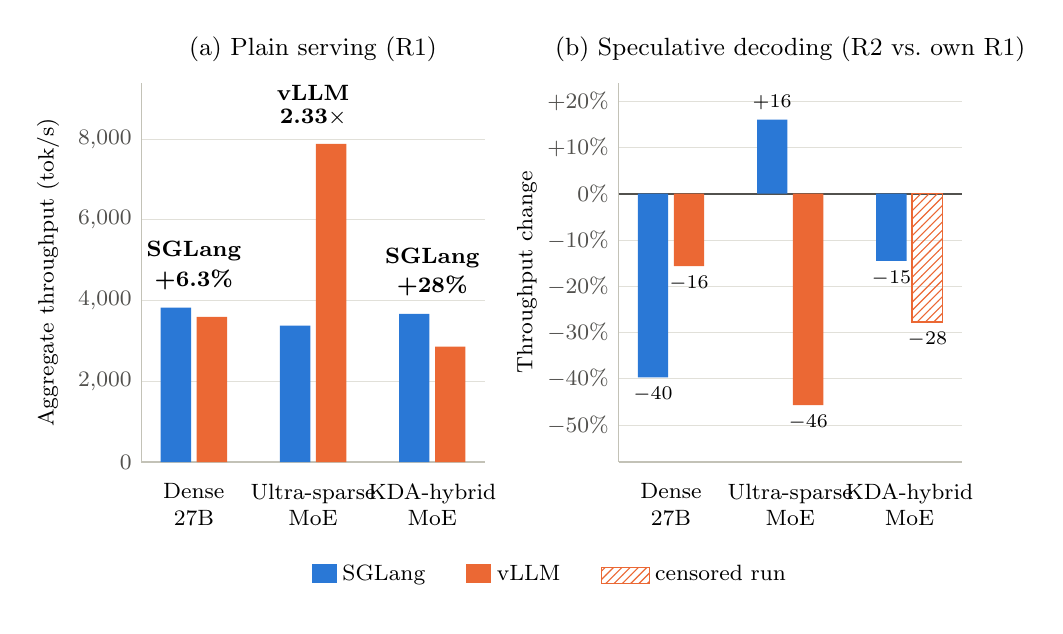
\begin{tikzpicture}
\begin{groupplot}[
  group style={group size=2 by 1, horizontal sep=1.7cm},
  width=0.49\textwidth, height=6.4cm,
  ybar, /pgf/bar width=11pt,
  symbolic x coords={Dense,MoE,KDA},
  xtick=data,
  xticklabels={{Dense\\27B},{Ultra-sparse\\MoE},{KDA-hybrid\\MoE}},
  xticklabel style={align=center, font=\footnotesize, text=black},
  enlarge x limits=0.22,
  axis lines*=left, axis line style={draw=axisc}, tick style={draw=none},
  ymajorgrids=true, grid style={draw=gridc, line width=0.3pt},
  yticklabel style={font=\footnotesize, text=inksec},
  ylabel style={font=\footnotesize},
  title style={font=\small, yshift=-2pt},
  legend style={draw=none, font=\footnotesize, legend columns=3,
                /tikz/every even column/.append style={column sep=0.45cm}},
  legend image code/.code={\draw[#1, draw=none] (0cm,-0.1cm) rectangle (0.32cm,0.14cm);},
]
% (a) R1 throughput: observed leader per model
\nextgroupplot[title={(a) Plain serving (R1)},
  ymin=0, ymax=9400, ytick={0,2000,4000,6000,8000}, yticklabels={0,2{,}000,4{,}000,6{,}000,8{,}000},
  clip=false,
  ylabel={Aggregate throughput (\tps)},
  legend to name=fwlegend]
\addplot[fill=sglang, draw=none, bar shift=-6.5pt] coordinates {(Dense,3823) (MoE,3383) (KDA,3669)};
\addlegendentry{SGLang}
\addplot[fill=vllm, draw=none, bar shift=6.5pt] coordinates {(Dense,3597) (MoE,7886) (KDA,2857)};
\addlegendentry{vLLM}
\addlegendimage{area legend, draw=vllm, pattern=north east lines, pattern color=vllm}
\addlegendentry{censored run}
\node[font=\footnotesize\bfseries, anchor=south] at (axis cs:Dense,3823) [yshift=3pt] {\shortstack{SGLang\\+6.3\%}};
\node[font=\footnotesize\bfseries, anchor=south] at (axis cs:MoE,7886) [yshift=3pt] {\shortstack{vLLM\\2.33$\times$}};
\node[font=\footnotesize\bfseries, anchor=south] at (axis cs:KDA,3669) [yshift=3pt] {\shortstack{SGLang\\+28\%}};
% (b) effect of speculative decoding, relative to the same framework's R1
\nextgroupplot[title={(b) Speculative decoding (R2 vs.\ own R1)},
  ymin=-58, ymax=24, ytick={-50,-40,-30,-20,-10,0,10,20},
  yticklabels={$-50\%$,$-40\%$,$-30\%$,$-20\%$,$-10\%$,0\%,$+10\%$,$+20\%$},
  ylabel={Throughput change}, ylabel shift=-3pt,
  nodes near coords={\pgfmathprintnumber[fixed,precision=0,showpos]{\pgfplotspointmeta}},
  nodes near coords align={vertical},
  every node near coord/.append style={font=\scriptsize, text=black},
  extra y ticks={0}, extra y tick labels={},
  extra y tick style={grid style={draw=inksec, line width=0.6pt}}]
\addplot[fill=sglang, draw=none, bar shift=-6.5pt] coordinates {(Dense,-39.68) (MoE,16.03) (KDA,-14.54)};
\addplot[fill=vllm, draw=none, bar shift=6.5pt] coordinates {(Dense,-15.67) (MoE,-45.71)};
\addplot[draw=vllm, line width=0.5pt, pattern=north east lines, pattern color=vllm, bar shift=6.5pt] coordinates {(KDA,-27.69)};
\end{groupplot}
\node[anchor=north] at ($(group c1r1.south)!0.5!(group c2r1.south)+(0,-1.05cm)$) {\pgfplotslegendfromname{fwlegend}};
\end{tikzpicture}
\caption{The three comparisons at a glance (values from Tables~\ref{tab:dense-r1}--\ref{tab:kda}). (a)~Plain-serving throughput; the label above each pair names the observed leader and its margin. (b)~Change in aggregate throughput when the checkpoint's speculative-decoding head is enabled, relative to the same framework's R1; five of six bars are below zero. SGLang's dense R2 also includes its automatic cap reduction from 128 to 48 (Section~\ref{sec:dense}). The hatched bar is a censored measurement: 85.6\% success, work truncated at 623k tokens (Section~\ref{sec:method}).}
\label{fig:throughput}
\end{figure}

\begin{table}[t]
\centering
\small
\begin{tabular}{llr@{\hspace{1.4em}}cc}
\toprule
 & & & \multicolumn{2}{c}{\textbf{R2 vs.\ own R1}} \\
\cmidrule(l){4-5}
\textbf{Architecture (model)} & \textbf{R1 leader} & \textbf{Margin} & \textbf{SGLang} & \textbf{vLLM} \\
\midrule
Dense hybrid (Qwen3.8-27B) & SGLang & +6.3\% & $-$40\%$^{a}$ & $-$16\% \\
Ultra-sparse MoE (Qwen3.8-Flash-Next) & vLLM & 2.33$\times$ & +16\% & $-$46\% \\
KDA-hybrid MoE (GLM-5.3-Flash) & SGLang & +28\% & $-$15\% & $-$28\%$^{b}$ \\
\bottomrule
\end{tabular}
\caption{Synthesis across the three comparisons. The last two columns give each framework's throughput change when speculative decoding is enabled. $^{a}$Includes SGLang's automatic cap reduction from 128 to 48 (Section~\ref{sec:dense}). $^{b}$Censored: 85.6\% success (Section~\ref{sec:method}). Framework versions as in Table~\ref{tab:conditions}: SGLang 0.5.20 throughout; vLLM 0.29.1rc1 on the dense and ultra-sparse MoE models; dedicated vLLM 0.28.1rc1 build on the KDA model.}
\label{tab:synthesis}
\end{table}

Two regularities stand out. First (Figure~\ref{fig:throughput}a), the framework gap was smallest on the well-trodden dense hybrid (6\%) and largest on the newer ultra-sparse MoE (2.3$\times$), which may reflect how recently each framework acquired mature kernels for a given architecture---though with one model per architecture we cannot separate this from framework-version and workload differences. Second (Figure~\ref{fig:throughput}b), in these runs \emph{speculative decoding behaved as a latency tool turned throughput cost at this concurrency}: in five of the six framework--model pairs, draft-and-verify FLOPs appear not to have been recovered by acceptance gains, consistent with decode batches already binding GPU capacity (we did not measure acceptance lengths or utilization). The single positive case (SGLang NEXTN on the 6B-active MoE) is consistent with this explanation---cheap decodes leave headroom for drafting---rather than contradicting it.

\subsection{Platform-level capacity and reliability}
\label{sec:reliability}

Beyond per-engine comparisons, the platform sustained a mixed workload of 1,500 concurrent users across all three engines with 100\% success, 8,146 \tps{} aggregate throughput, and 76.8 s P95 from the fronting VM through the tunnel and gateway (Table~\ref{tab:reliability}). Gateway overhead at this load was 2.5\% CPU and 405 MB of memory, and no gateway-related failures were observed at the tested burst size; per-layer latency was not measured, so this does not rule out a throughput limit in the gateway.

\begin{table}[t]
\centering
\footnotesize
\begin{tabularx}{\textwidth}{>{\raggedright\arraybackslash}Xccc>{\raggedright\arraybackslash}p{4.9cm}}
\toprule
\textbf{Stage of the reliability investigation} & \textbf{Success} & \textbf{Aggregate} & \textbf{P95} & \textbf{Root cause identified} \\
\midrule
Initial mixed run (1,500 users) & 67.9\% & --- & --- & Client shell \texttt{ulimit -n} 1024 $\rightarrow$ fd exhaustion (Errno 24) at $\sim$1,020 open sockets \\
After client fix, via tunnel & 91.8\% & 8,251 \tps & 70.4 s & Per-connection sshd on the tunnel VM also capped at 1024 fds (verified via \texttt{/proc/<pid>/limits}) \\
Bypassing the tunnel (direct) & 100\% & 8,156 \tps & 77.6 s & Isolated remaining losses to the VM$\leftrightarrow$gateway segment \\
After \texttt{/etc/security/limits.conf} fix, via tunnel & \textbf{100\%} & 8,146 \tps & 76.8 s & Correct fix: PAM \texttt{limits.conf} (systemd override alone does not apply to per-connection sshd); tunnel re-established after the fix \\
\bottomrule
\end{tabularx}
\caption{Layered attribution of mixed-load failures (1,500 users $\times$ 500 tokens; three engines live).}
\label{tab:reliability}
\end{table}

We report this debugging arc as a result in its own right for two reasons. First, an initial hypothesis---that an 8\% ReadError rate indicated a single-flow ceiling of the reverse tunnel---was \emph{refuted} by the fix-and-remeasure cycle: after correcting both fd limits, 1,500 concurrent users traversed the single tunnel flow at 100\% success, so no such ceiling was reached below 1,500. Second, the diagnosis illustrates a methodology we now apply routinely: measure each layer independently (client $\rightarrow$ tunnel $\rightarrow$ gateway $\rightarrow$ engine), fix one layer at a time, and re-run the identical workload after each fix rather than trusting bypass experiments to localize faults finer than segment granularity.

\section{Discussion}

\textbf{Framework choice is a per-model decision, and it is large.} The observed spread---from a 6\% margin to a 2.33$\times$ gap---is the largest lever we measured on correctly configured engines. Concurrency-cap tuning, in separate measurements on the same engines, moved throughput by 29--39\% (raising the KDA engine's cap from 64 to 128 gained 31\% and lifted success from 95.7\% to 100\%; raising the MoE engine's cap from 48 to 100 gained 29\% on average throughput and 39\% on peak); the two embedding-placement configurations differed by 2.6\% in single runs; and restoring a misconfigured SGLang baseline on the dense engine had earlier been worth +48\%. In operational terms, choosing the wrong framework for the ultra-sparse MoE would have cost more throughput than any misconfiguration of a correctly chosen framework. The practical implication we adopted institutionally is a \emph{dual-framework onboarding policy}: every new model is deployed on both frameworks under suffixed aliases, A/B-tested under the production workload, and promoted by a two-line configuration change; the platform of Section~\ref{sec:platform} makes this a routine procedure rather than a redeployment project. We recommend this as default practice for multi-model serving platforms.

\textbf{Speculative decoding at high concurrency.} Our results add same-checkpoint evidence from a production platform to a phenomenon that goodput analyses have already identified: when speculation is applied without regard to load, its verification FLOPs compete with useful work and acceptance gains cannot pay for them~\cite{liu2024turbospec}. Under 500--1,000 concurrent users, with decode batches that appeared to saturate GPU capacity, this cost appeared in five of six pairs, and in the worst case the added per-request time pushed 14.4\% of requests past the 300 s client timeout setting. Adaptive systems such as TurboSpec address this by gating speculation on measured goodput~\cite{liu2024turbospec}, and AdaServe by customizing it to per-request SLOs~\cite{li2025adaserve}; our measurements suggest a cruder but zero-engineering-cost policy---disable integrated MTP/NEXTN for short-prompt, high-concurrency throughput serving of these architectures---captures most of the benefit we observed. We do \emph{not} conclude that speculative decoding is useless: at low concurrency, for single-stream latency, or---per MagicDec's analysis---for long contexts under high batch~\cite{sadhukhan2024magicdec} it can remain appropriate, and the one positive case here (SGLang NEXTN, +16\% at 6B active parameters) is consistent with a model-dependent crossover, as in the goodput formulation~\cite{liu2024turbospec}, although our runs did not isolate its cause. The decision should be made from a measurement at the deployment's own concurrency, not from the feature's reputation.

\textbf{Memory accounting can decide speculative feasibility.} A secondary observation: the two frameworks' speculative implementations have very different memory profiles on hybrid-attention models. On the dense hybrid, SGLang's EAGLE loads the draft weights plus a 13.8 GB intermediate-state cache, and the framework automatically reduces the concurrency cap from 128 to 48 when speculative decoding is enabled (Section~\ref{sec:dense}); vLLM's MTP shares the head weights within the checkpoint and preserved the cap. On models whose caches dominate memory, this implementation difference alone can outweigh acceptance-rate considerations, and it is invisible in feature lists.

\textbf{Dedicated builds and version governance.} The KDA comparison could not be run on the generic vLLM nightly at all (kernel assertion; autotuning hang), while the vendor's dedicated build ran correctly. Our resulting policy---version-named images that are not overwritten by default, dedicated builds preferred when they exist, ``once supported $\ne$ always supported''---converted what could have been days of kernel-level debugging into a one-line image selection. We note this as a reproducibility point: framework \emph{version} is a first-class experimental variable on new architectures, and evaluations that do not pin and report it are hard to reproduce. A version name is not a content identity, however: we did not record OCI digests or SIF checksums for the images used here, so the tested builds are identified only by name and build string (\texttt{engines/KNOWN\_GOOD.md}).

\textbf{What the platform measurements do and do not show.} The layered analysis of Section~\ref{sec:reliability} observed no additional gateway- or tunnel-related failures at the tested burst size: the gateway used 2.5\% CPU at 1,500 users, and no single-flow tunnel ceiling was observed below 1,500 users. These runs did not pass through the TLS front end and include no capacity sweep, GPU-utilization data, or per-layer latency breakdown, so they do not establish where the next bottleneck lies or characterize the capacity of the TLS tier.

\textbf{Agents as experimentalists.} Beyond its findings, this study is a working example of an LLM-based agent assisting with an experimental procedure under human approval. Autonomous research agents have been demonstrated for closed-loop scientific discovery~\cite{lu2024aiscientist}; agent-driven simulation has been proposed to track the fast-moving serving design space because real deployments are costly~\cite{kim2026simthesizer}; and AutoTuneBench has agent systems auto-tune both engines under a measurement protocol stricter than ours~\cite{chen2026autotunebench}. Our pipeline is closest to the last of these but different in object: AutoTuneBench tunes engine configurations, whereas our skills drive the full production lifecycle---deployment behind a live gateway, benchmarking through the external traffic path, verdict recording, and production traffic switching---on infrastructure that keeps serving users throughout.

What made the automation trustworthy was not the agent's raw capability but the enclosure: declarative skills that require documentation-traceable configuration, machine-checked output-token comparisons, traffic isolation that makes candidate engines harmless to production, and mandatory evidence journaling from which this paper's tables are extracted. Within that enclosure, the agent performed work that would otherwise gate on scarce systems-engineering time; the repository's commit history records all three verdicts on 2026-09-27, with the vLLM counterpart engines scaffolded the same day (the SGLang engines already served production traffic), although we did not measure unattended time or labor savings; the same enclosure makes the next framework decision a documented procedure rather than an ad hoc project. The pattern extends to the manuscript itself: the literature search and citation verification (identifiers and author lists checked against the arXiv API; residual errors were caught in external review), the structural drafting from writing-methodology skills, and the evidence-alignment audit were likewise agent-performed. Related benchmarks evaluate how well agents do DevOps tasks~\cite{tang2026devopsgym}; here the DevOps task itself---deploying, benchmarking, and switching production inference infrastructure---was the experiment. We take this as an operational answer to the question this paper opened with: ``which framework should serve this model?'' is better answered by a measurement whose procedure is a versioned artifact of the repository than by folklore or release notes.

\section{Limitations and Future Work}

Three limitations bound the strength of our conclusions. First, each configuration was measured once at a single workload shape (uniform concurrency, uniform max\_tokens); we did not measure variance across repeats, so no margin here is an established effect, and the dense comparison's $+$6.3\% should be read as near parity. The workload is a single-burst queue drain---all requests are released at once over a pool of five short prompts---so latency percentiles largely reflect queue-drain time rather than steady-state request latency, and P95 should not be read as an SLO metric. Two R2 results carry additional confounds we flag rather than resolve: SGLang's dense R2 combines speculative decoding with the framework's automatic cap reduction to 48 (no cap-48 plain control was run), and KDA vLLM's R2 is censored by client timeouts (Section~\ref{sec:method}). Scheduler placement also put some A/B pairs on different nodes of the cluster. We further did not measure streaming latency---time to first token (TTFT) and time per output token (TPOT)---under open-loop arrivals, did not sweep concurrency to locate the speculative-decoding crossover, and did not record acceptance lengths or GPU utilization---so the mechanism attributions in Section~5 remain hypotheses. The harness stores per-run summary statistics only: it records no per-request lengths, finish reasons, or outputs, sets no sampling seed, and runs no output-quality check, and the prefix-cache and warm-up state of each engine was not controlled. The measurements also did not include the TLS front end, and we did not record the checkpoint revisions, tokenizer or chat-template versions, or image digests used in each run. Second, framework versions evolve monthly; our results pin SGLang 0.5.20 and vLLM 0.29.1rc1 (plus a dedicated 0.28.1rc1 build for the KDA model), and the ultra-sparse MoE gap in particular should be expected to narrow or move as kernels mature. Third, all measurements are single-engine deployments on one cluster; multi-instance load-balanced configurations were validated only for success rate (Section~\ref{sec:reliability}), not A/B-compared.

Future work should extend the matrix in six directions: repeat runs with confidence intervals and mixed workload shapes; add FP8-versus-BF16 and KV-cache-dtype axes, which our Hopper hardware partially constrains for the KDA model (FP8 KV unsupported); test whether the observed MoE framework gap closes in later SGLang releases, which would calibrate how quickly such evaluations expire; measure streaming TTFT/TPOT under open-loop arrivals; sweep concurrency to locate the speculative-decoding crossover, recording acceptance lengths; and profile GPU utilization and MoE kernel time to test the mechanism attributions offered in Section~5.

\section{Conclusion}

We built a multi-model API service on an HPC cluster---a LiteLLM gateway over Slurm-managed engines on H200 GPUs---and, confronted with the recurring question of which serving framework to assign to each new model, encoded the comparison procedure as versioned skills that an LLM-based agent executed under human approval: scaffold both frameworks from official documentation, deploy under traffic-isolated aliases, benchmark both under the same workload with output-token counts compared, record the verdict, and switch production traffic when warranted. Applied to three architecturally distinct LLMs, the agent-assisted comparisons found that the leading framework changed with each model---SGLang +6.3\% (near parity) on a dense hybrid, vLLM by 2.33$\times$ on an ultra-sparse MoE, SGLang +28\% on a KDA-hybrid MoE---and that speculative decoding on the same checkpoints reduced measured throughput in five of six framework--model pairs (single-run measurements), a verdict applied to production the same day it was measured. The same agent-assisted workflow diagnosed a mixed-load reliability fault from an encoded symptom-to-cause procedure, raising success from 67.9\% to 100\%. Together, the results argue for treating framework selection and speculative decoding not as defaults to be inherited but as per-model, per-workload decisions---and for making the measurement that informs them cheap and safe enough to run on every new model, which is the purpose of the agent-assisted procedure described here.

\section*{AI-Use Disclosure}

\textbf{Research execution.} The experiments reported in this paper---engine deployment, benchmarking, failure diagnosis, and production traffic switching---were executed by LLM-based coding agents following the versioned procedures (``skills'') described in Section~\ref{sec:platform}, under the direction and release decisions of the human authors.

\textbf{Literature search and verification.} The literature search, and the verification of every arXiv identifier and author list, were performed by an agent against the arXiv API. This process had a disclosed failure mode: an intermediate reference-conversion pass introduced incorrect author lists in five entries, which were caught and corrected during independent external review---a known transcription-error class for AI-assisted literature verification. Responsibility for reference accuracy rests with the authors.

\textbf{Manuscript drafting.} The drafting and revision of this manuscript, including structural drafting from writing-methodology skills, evidence-alignment auditing, the LaTeX conversion, and BibTeX generation, were produced by agents from the underlying machine-recorded results; the agent used for the initial drafting and text revisions was opencode, powered by GLM-5.3. A second LLM agent, Claude Code (Anthropic Claude Opus 5.5), performed eight rounds of external review (three adversarial content reviews, three pre-submission checks, and two regression checks) whose findings are incorporated above; after the reviews, the same agent redrew Figures~\ref{fig:arch} and~\ref{fig:throughput} and revised Tables~\ref{tab:moe}--\ref{tab:reliability}, without changing any reported value. A third model, GPT-6 (ASTRA), then produced an independent external review; in response, Claude Code revised the text to narrow claims to the evidence---including the title, abstract, contributions, the benchmark path in Figure~\ref{fig:arch}, and the limitations---without adding experiments or changing any reported value, and GPT-6 reviewed those revisions in two further regression rounds.

\textbf{Human role.} Problem framing, platform and release decisions, and verdict approval were made by the human authors, who also secured the funding. The corresponding author is responsible for final verification of the principal numerical results, calculations, and claim--citation links.

\textbf{A disclosed limit of this disclosure.} The experimental phases ran across multiple agent sessions whose verbatim prompts and model versions were not preserved as timestamped transcripts; the skills, engine configurations, raw result files, job records, and commit history are released, but this disclosure cannot provide call-by-call detail. Consistent with arXiv and conference policy, no AI system is listed as an author, and the human authors take full responsibility for the manuscript's content.

\section*{Author Contributions}

\textbf{Chao-Chun Chuang:} Conceptualization, Methodology, Software, Investigation, Formal analysis, and Writing --- original draft. \textbf{Po-Hsiang Lin:} Investigation, Data curation, Validation, and Writing --- review and editing.

\section*{Funding}

\begin{sloppypar}
This work was supported in part by the National Science and Technology Council (NSTC), Taiwan, under Grant Nos.\ NSTC 115-2410-H-A49-046-MY3 and NSTC 114-2634-F-006-002.
\end{sloppypar}

\section*{Competing Interests}

The authors declare that they have no competing interests.

\section*{Acknowledgments}

The authors gratefully acknowledge the National Center for High-performance Computing (NCHC), National Institutes of Applied Research (NIAR), Taiwan, for providing the research resources, computational infrastructure, and platform services that supported this work.

\section*{Data and Artifact Availability}

The platform repository is available at \url{https://github.com/gemini960114/litellm-proxy}. Raw per-run statistics (JSON) for all configurations in Tables~\ref{tab:dense-r1}--\ref{tab:reliability}---except the initial 67.9\% mixed run, which is recorded in the platform's operations documentation---are available in its \texttt{benchmarks/\allowbreak results/} directory. Engine configurations are recorded in \texttt{engines/KNOWN\_GOOD.md}. The evaluation skills (model-onboarding, concurrency-troubleshooting, debug-journaling) are released with the platform repository (\texttt{.agents/skills/}). The manuscript-writing skills are third-party skills that the repository pins by content hash in \texttt{skills-lock.json} but does not redistribute. The repository is a substantial but not complete replication package: it does not redistribute the model checkpoints or the multi-gigabyte container images (referenced by version names, not content digests), and it does not preserve the agent sessions' verbatim prompts.

\bibliographystyle{unsrtnat}
\bibliography{refs}

\end{document}
